\documentclass[12pt]{article}

%packages
%\usepackage{latexsym}
\usepackage{graphicx}
\usepackage{color}
\usepackage{amsmath}
\usepackage{dsfont}
\usepackage{placeins}
\usepackage{amssymb}
\usepackage{wasysym}
\usepackage{abstract}
\usepackage{hyperref}
\usepackage{etoolbox}
\usepackage{datetime}
\usepackage{xcolor}
\usepackage{alphalph}
\settimeformat{ampmtime}

%\usepackage{pstricks,pst-node,pst-tree}

%\usepackage{algpseudocode}
%\usepackage{amsthm}
%\usepackage{hyperref}
%\usepackage{mathrsfs}
%\usepackage{amsfonts}
%\usepackage{bbding}
%\usepackage{listings}
%\usepackage{appendix}
\usepackage[margin=1in]{geometry}
%\geometry{papersize={8.5in,11in},total={6.5in,9in}}
%\usepackage{cancel}
%\usepackage{algorithmic, algorithm}

\makeatletter
\def\maxwidth{ %
  \ifdim\Gin@nat@width>\linewidth
    \linewidth
  \else
    \Gin@nat@width
  \fi
}
\makeatother

\definecolor{fgcolor}{rgb}{0.345, 0.345, 0.345}
\newcommand{\hlnum}[1]{\textcolor[rgb]{0.686,0.059,0.569}{#1}}%
\newcommand{\hlstr}[1]{\textcolor[rgb]{0.192,0.494,0.8}{#1}}%
\newcommand{\hlcom}[1]{\textcolor[rgb]{0.678,0.584,0.686}{\textit{#1}}}%
\newcommand{\hlopt}[1]{\textcolor[rgb]{0,0,0}{#1}}%
\newcommand{\hlstd}[1]{\textcolor[rgb]{0.345,0.345,0.345}{#1}}%
\newcommand{\hlkwa}[1]{\textcolor[rgb]{0.161,0.373,0.58}{\textbf{#1}}}%
\newcommand{\hlkwb}[1]{\textcolor[rgb]{0.69,0.353,0.396}{#1}}%
\newcommand{\hlkwc}[1]{\textcolor[rgb]{0.333,0.667,0.333}{#1}}%
\newcommand{\hlkwd}[1]{\textcolor[rgb]{0.737,0.353,0.396}{\textbf{#1}}}%

\usepackage{framed}
\makeatletter
\newenvironment{kframe}{%
 \def\at@end@of@kframe{}%
 \ifinner\ifhmode%
  \def\at@end@of@kframe{\end{minipage}}%
  \begin{minipage}{\columnwidth}%
 \fi\fi%
 \def\FrameCommand##1{\hskip\@totalleftmargin \hskip-\fboxsep
 \colorbox{shadecolor}{##1}\hskip-\fboxsep
     % There is no \\@totalrightmargin, so:
     \hskip-\linewidth \hskip-\@totalleftmargin \hskip\columnwidth}%
 \MakeFramed {\advance\hsize-\width
   \@totalleftmargin\z@ \linewidth\hsize
   \@setminipage}}%
 {\par\unskip\endMakeFramed%
 \at@end@of@kframe}
\makeatother

\definecolor{shadecolor}{rgb}{.77, .77, .77}
\definecolor{messagecolor}{rgb}{0, 0, 0}
\definecolor{warningcolor}{rgb}{1, 0, 1}
\definecolor{errorcolor}{rgb}{1, 0, 0}
\newenvironment{knitrout}{}{} % an empty environment to be redefined in TeX

\usepackage{alltt}
\usepackage[T1]{fontenc}

\newcommand{\qu}[1]{``#1''}
\newcounter{probnum}
\setcounter{probnum}{1}

%create definition to allow local margin changes
\def\changemargin#1#2{\list{}{\rightmargin#2\leftmargin#1}\item[]}
\let\endchangemargin=\endlist 

%allow equations to span multiple pages
\allowdisplaybreaks

%define colors and color typesetting conveniences
\definecolor{gray}{rgb}{0.5,0.5,0.5}
\definecolor{black}{rgb}{0,0,0}
\definecolor{white}{rgb}{1,1,1}
\definecolor{blue}{rgb}{0.5,0.5,1}
\newcommand{\inblue}[1]{\color{blue}#1 \color{black}}
\definecolor{green}{rgb}{0.133,0.545,0.133}
\newcommand{\ingreen}[1]{\color{green}#1 \color{black}}
\definecolor{yellow}{rgb}{1,1,0}
\newcommand{\inyellow}[1]{\color{yellow}#1 \color{black}}
\definecolor{orange}{rgb}{0.9,0.649,0}
\newcommand{\inorange}[1]{\color{orange}#1 \color{black}}
\definecolor{red}{rgb}{1,0.133,0.133}
\newcommand{\inred}[1]{\color{red}#1 \color{black}}
\definecolor{purple}{rgb}{0.58,0,0.827}
\newcommand{\inpurple}[1]{\color{purple}#1 \color{black}}
\definecolor{backgcode}{rgb}{0.97,0.97,0.8}
\definecolor{Brown}{cmyk}{0,0.81,1,0.60}
\definecolor{OliveGreen}{cmyk}{0.64,0,0.95,0.40}
\definecolor{CadetBlue}{cmyk}{0.62,0.57,0.23,0}

%define new math operators
\DeclareMathOperator*{\argmax}{arg\,max~}
\DeclareMathOperator*{\argmin}{arg\,min~}
\DeclareMathOperator*{\argsup}{arg\,sup~}
\DeclareMathOperator*{\arginf}{arg\,inf~}
\DeclareMathOperator*{\convolution}{\text{\Huge{$\ast$}}}
\newcommand{\infconv}[2]{\convolution^\infty_{#1 = 1} #2}
%true functions

%%%% GENERAL SHORTCUTS

%shortcuts for pure typesetting conveniences
\newcommand{\bv}[1]{\boldsymbol{#1}}

%shortcuts for compound constants
\newcommand{\BetaDistrConst}{\dfrac{\Gamma(\alpha + \beta)}{\Gamma(\alpha)\Gamma(\beta)}}
\newcommand{\NormDistrConst}{\dfrac{1}{\sqrt{2\pi\sigma^2}}}

%shortcuts for conventional symbols
\newcommand{\tsq}{\tau^2}
\newcommand{\tsqh}{\hat{\tau}^2}
\newcommand{\sigsq}{\sigma^2}
\newcommand{\sigsqsq}{\parens{\sigma^2}^2}
\newcommand{\sigsqovern}{\dfrac{\sigsq}{n}}
\newcommand{\tausq}{\tau^2}
\newcommand{\tausqalpha}{\tau^2_\alpha}
\newcommand{\tausqbeta}{\tau^2_\beta}
\newcommand{\tausqsigma}{\tau^2_\sigma}
\newcommand{\betasq}{\beta^2}
\newcommand{\sigsqvec}{\bv{\sigma}^2}
\newcommand{\sigsqhat}{\hat{\sigma}^2}
\newcommand{\sigsqhatmlebayes}{\sigsqhat_{\text{Bayes, MLE}}}
\newcommand{\sigsqhatmle}[1]{\sigsqhat_{#1, \text{MLE}}}
\newcommand{\bSigma}{\bv{\Sigma}}
\newcommand{\bSigmainv}{\bSigma^{-1}}
\newcommand{\thetavec}{\bv{\theta}}
\newcommand{\thetahat}{\hat{\theta}}
\usepackage{accents}
\newlength{\dhatheight}
\newcommand{\doublehat}[1]{%
    \settoheight{\dhatheight}{\ensuremath{\hat{#1}}}%
    \addtolength{\dhatheight}{-0.35ex}%
    \hat{\vphantom{\rule{1pt}{\dhatheight}}%
    \smash{\hat{#1}}}}

\newcommand{\thetahathat}{\doublehat{\theta}}
\newcommand{\thetahatmle}{\hat{\theta}_{\mathrm{MLE}}}
\newcommand{\thetavechatmle}{\hat{\thetavec}_{\mathrm{MLE}}}
\newcommand{\muhat}{\hat{\mu}}
\newcommand{\musq}{\mu^2}
\newcommand{\muvec}{\bv{\mu}}
\newcommand{\muhatmle}{\muhat_{\text{MLE}}}
\newcommand{\lambdahat}{\hat{\lambda}}
\newcommand{\lambdahatmle}{\lambdahat_{\text{MLE}}}
\newcommand{\etavec}{\bv{\eta}}
\newcommand{\alphavec}{\bv{\alpha}}
\newcommand{\minimaxdec}{\delta^*_{\mathrm{mm}}}
\newcommand{\ybar}{\bar{y}}
\newcommand{\xbar}{\bar{x}}
\newcommand{\Xbar}{\bar{X}}
\newcommand{\phat}{\hat{p}}
\newcommand{\Phat}{\hat{P}}
\newcommand{\Zbar}{\bar{Z}}
\newcommand{\iid}{~{\buildrel iid \over \sim}~}
\newcommand{\inddist}{~{\buildrel ind \over \sim}~}
\newcommand{\approxdist}{~{\buildrel approx \over \sim}~}
\newcommand{\equalsindist}{~{\buildrel d \over =}~}
\newcommand{\loglik}[1]{\ell\parens{#1}}
\newcommand{\thetahatkminone}{\thetahat^{(k-1)}}
\newcommand{\thetahatkplusone}{\thetahat^{(k+1)}}
\newcommand{\thetahatk}{\thetahat^{(k)}}
\newcommand{\half}{\frac{1}{2}}
\newcommand{\third}{\frac{1}{3}}
\newcommand{\twothirds}{\frac{2}{3}}
\newcommand{\fourth}{\frac{1}{4}}
\newcommand{\fifth}{\frac{1}{5}}
\newcommand{\sixth}{\frac{1}{6}}

%shortcuts for vector and matrix notation
\newcommand{\A}{\bv{A}}
\newcommand{\At}{\A^T}
\newcommand{\Ainv}{\inverse{\A}}
\newcommand{\B}{\bv{B}}
\newcommand{\K}{\bv{K}}
\newcommand{\Kt}{\K^T}
\newcommand{\Kinv}{\inverse{K}}
\newcommand{\Kinvt}{(\Kinv)^T}
\newcommand{\M}{\bv{M}}
\newcommand{\Bt}{\B^T}
\newcommand{\Q}{\bv{Q}}
\newcommand{\Qt}{\Q^T}
\newcommand{\R}{\bv{R}}
\newcommand{\Rt}{\R^T}
\newcommand{\Z}{\bv{Z}}
\newcommand{\X}{\bv{X}}
\newcommand{\Xsub}{\X_{\text{(sub)}}}
\newcommand{\Xsubadj}{\X_{\text{(sub,adj)}}}
\newcommand{\I}{\bv{I}}
\newcommand{\Y}{\bv{Y}}
\newcommand{\T}{\bv{T}}
\newcommand{\sigsqI}{\sigsq\I}
\renewcommand{\P}{\bv{P}}
\newcommand{\Psub}{\P_{\text{(sub)}}}
\newcommand{\Pt}{\P^T}
\newcommand{\Pii}{P_{ii}}
\newcommand{\Pij}{P_{ij}}
\newcommand{\IminP}{(\I-\P)}
\newcommand{\Xt}{\bv{X}^T}
\newcommand{\XtX}{\Xt\X}
\newcommand{\XtXinv}{\parens{\Xt\X}^{-1}}
\newcommand{\XtXinvXt}{\XtXinv\Xt}
\newcommand{\XXtXinvXt}{\X\XtXinvXt}
\newcommand{\x}{\bv{x}}
\newcommand{\p}{\bv{p}}
\newcommand{\onevec}{\bv{1}}
\newcommand{\oneton}{1, \ldots, n}
\newcommand{\yoneton}{y_1, \ldots, y_n}
\newcommand{\yonetonorder}{y_{(1)}, \ldots, y_{(n)}}
\newcommand{\Yoneton}{Y_1, \ldots, Y_n}
\newcommand{\iinoneton}{i \in \braces{\oneton}}
\newcommand{\onetom}{1, \ldots, m}
\newcommand{\jinonetom}{j \in \braces{\onetom}}
\newcommand{\xoneton}{x_1, \ldots, x_n}
\newcommand{\Xoneton}{X_1, \ldots, X_n}
\newcommand{\xt}{\x^T}
\newcommand{\y}{\bv{y}}
\newcommand{\yt}{\y^T}
\renewcommand{\c}{\bv{c}}
\newcommand{\ct}{\c^T}
\newcommand{\tstar}{\bv{t}^*}
\renewcommand{\u}{\bv{u}}
\renewcommand{\v}{\bv{v}}
\renewcommand{\a}{\bv{a}}
\newcommand{\s}{\bv{s}}
\newcommand{\yadj}{\y_{\text{(adj)}}}
\newcommand{\xjadj}{\x_{j\text{(adj)}}}
\newcommand{\xjadjM}{\x_{j \perp M}}
\newcommand{\yhat}{\hat{\y}}
\newcommand{\yhatsub}{\yhat_{\text{(sub)}}}
\newcommand{\yhatstar}{\yhat^*}
\newcommand{\yhatstarnew}{\yhatstar_{\text{new}}}
\newcommand{\z}{\bv{z}}
\newcommand{\zt}{\z^T}
\newcommand{\bb}{\bv{b}}
\newcommand{\bbt}{\bb^T}
\newcommand{\bbeta}{\bv{\beta}}
\newcommand{\beps}{\bv{\epsilon}}
\newcommand{\bepst}{\beps^T}
\newcommand{\e}{\bv{e}}
\newcommand{\Mofy}{\M(\y)}
\newcommand{\KofAlpha}{K(\alpha)}
\newcommand{\ellset}{\mathcal{L}}
\newcommand{\oneminalph}{1-\alpha}
\newcommand{\SSE}{\text{SSE}}
\newcommand{\SSEsub}{\text{SSE}_{\text{(sub)}}}
\newcommand{\MSE}{\text{MSE}}
\newcommand{\RMSE}{\text{RMSE}}
\newcommand{\SSR}{\text{SSR}}
\newcommand{\SST}{\text{SST}}
\newcommand{\JSest}{\delta_{\text{JS}}(\x)}
\newcommand{\Bayesest}{\delta_{\text{Bayes}}(\x)}
\newcommand{\EmpBayesest}{\delta_{\text{EmpBayes}}(\x)}
\newcommand{\BLUPest}{\delta_{\text{BLUP}}}
\newcommand{\MLEest}[1]{\hat{#1}_{\text{MLE}}}

%shortcuts for Linear Algebra stuff (i.e. vectors and matrices)
\newcommand{\twovec}[2]{\bracks{\begin{array}{c} #1 \\ #2 \end{array}}}
\newcommand{\threevec}[3]{\bracks{\begin{array}{c} #1 \\ #2 \\ #3 \end{array}}}
\newcommand{\fivevec}[5]{\bracks{\begin{array}{c} #1 \\ #2 \\ #3 \\ #4 \\ #5 \end{array}}}
\newcommand{\twobytwomat}[4]{\bracks{\begin{array}{cc} #1 & #2 \\ #3 & #4 \end{array}}}
\newcommand{\threebytwomat}[6]{\bracks{\begin{array}{cc} #1 & #2 \\ #3 & #4 \\ #5 & #6 \end{array}}}

%shortcuts for conventional compound symbols
\newcommand{\thetainthetas}{\theta \in \Theta}
\newcommand{\reals}{\mathbb{R}}
\newcommand{\complexes}{\mathbb{C}}
\newcommand{\rationals}{\mathbb{Q}}
\newcommand{\integers}{\mathbb{Z}}
\newcommand{\naturals}{\mathbb{N}}
\newcommand{\forallninN}{~~\forall n \in \naturals}
\newcommand{\forallxinN}[1]{~~\forall #1 \in \reals}
\newcommand{\matrixdims}[2]{\in \reals^{\,#1 \times #2}}
\newcommand{\inRn}[1]{\in \reals^{\,#1}}
\newcommand{\mathimplies}{\quad\Rightarrow\quad}
\newcommand{\mathlogicequiv}{\quad\Leftrightarrow\quad}
\newcommand{\eqncomment}[1]{\quad \text{(#1)}}
\newcommand{\limitn}{\lim_{n \rightarrow \infty}}
\newcommand{\limitN}{\lim_{N \rightarrow \infty}}
\newcommand{\limitd}{\lim_{d \rightarrow \infty}}
\newcommand{\limitt}{\lim_{t \rightarrow \infty}}
\newcommand{\limitsupn}{\limsup_{n \rightarrow \infty}~}
\newcommand{\limitinfn}{\liminf_{n \rightarrow \infty}~}
\newcommand{\limitk}{\lim_{k \rightarrow \infty}}
\newcommand{\limsupn}{\limsup_{n \rightarrow \infty}}
\newcommand{\limsupk}{\limsup_{k \rightarrow \infty}}
\newcommand{\floor}[1]{\left\lfloor #1 \right\rfloor}
\newcommand{\ceil}[1]{\left\lceil #1 \right\rceil}

%shortcuts for environments
\newcommand{\beqn}{\vspace{-0.25cm}\begin{eqnarray*}}
\newcommand{\eeqn}{\end{eqnarray*}}
\newcommand{\bneqn}{\vspace{-0.25cm}\begin{eqnarray}}
\newcommand{\eneqn}{\end{eqnarray}}

%shortcuts for mini environments
\newcommand{\parens}[1]{\left(#1\right)}
\newcommand{\squared}[1]{\parens{#1}^2}
\newcommand{\tothepow}[2]{\parens{#1}^{#2}}
\newcommand{\prob}[1]{\mathbb{P}\parens{#1}}
\newcommand{\cprob}[2]{\prob{#1~|~#2}}
\newcommand{\littleo}[1]{o\parens{#1}}
\newcommand{\bigo}[1]{O\parens{#1}}
\newcommand{\Lp}[1]{\mathbb{L}^{#1}}
\renewcommand{\arcsin}[1]{\text{arcsin}\parens{#1}}
\newcommand{\prodonen}[2]{\bracks{\prod_{#1=1}^n #2}}
\newcommand{\mysum}[4]{\sum_{#1=#2}^{#3} #4}
\newcommand{\sumonen}[2]{\sum_{#1=1}^n #2}
\newcommand{\infsum}[2]{\sum_{#1=1}^\infty #2}
\newcommand{\infprod}[2]{\prod_{#1=1}^\infty #2}
\newcommand{\infunion}[2]{\bigcup_{#1=1}^\infty #2}
\newcommand{\infinter}[2]{\bigcap_{#1=1}^\infty #2}
\newcommand{\infintegral}[2]{\int^\infty_{-\infty} #2 ~\text{d}#1}
\newcommand{\supthetas}[1]{\sup_{\thetainthetas}\braces{#1}}
\newcommand{\bracks}[1]{\left[#1\right]}
\newcommand{\braces}[1]{\left\{#1\right\}}
\newcommand{\set}[1]{\left\{#1\right\}}
\newcommand{\abss}[1]{\left|#1\right|}
\newcommand{\norm}[1]{\left|\left|#1\right|\right|}
\newcommand{\normsq}[1]{\norm{#1}^2}
\newcommand{\inverse}[1]{\parens{#1}^{-1}}
\newcommand{\rowof}[2]{\parens{#1}_{#2\cdot}}

%shortcuts for functionals
\newcommand{\realcomp}[1]{\text{Re}\bracks{#1}}
\newcommand{\imagcomp}[1]{\text{Im}\bracks{#1}}
\newcommand{\range}[1]{\text{range}\bracks{#1}}
\newcommand{\colsp}[1]{\text{colsp}\bracks{#1}}
\newcommand{\rowsp}[1]{\text{rowsp}\bracks{#1}}
\newcommand{\tr}[1]{\text{tr}\bracks{#1}}
\newcommand{\rank}[1]{\text{rank}\bracks{#1}}
\newcommand{\proj}[2]{\text{Proj}_{#1}\bracks{#2}}
\newcommand{\projcolspX}[1]{\text{Proj}_{\colsp{\X}}\bracks{#1}}
\newcommand{\median}[1]{\text{median}\bracks{#1}}
\newcommand{\mean}[1]{\text{mean}\bracks{#1}}
\newcommand{\dime}[1]{\text{dim}\bracks{#1}}
\renewcommand{\det}[1]{\text{det}\bracks{#1}}
\newcommand{\expe}[1]{\mathbb{E}\bracks{#1}}
\newcommand{\expeabs}[1]{\expe{\abss{#1}}}
\newcommand{\expesub}[2]{\mathbb{E}_{#1}\bracks{#2}}
\newcommand{\indic}[1]{\mathds{1}_{#1}}
\newcommand{\var}[1]{\mathbb{V}\text{ar}\bracks{#1}}
\newcommand{\cov}[2]{\mathbb{C}\text{ov}\bracks{#1, #2}}
\newcommand{\corrtwo}[2]{\text{Corr}\bracks{#1, #2}}
\newcommand{\corr}[1]{\text{Corr}\bracks{#1}}
\newcommand{\se}[1]{\mathbb{S}\text{E}\bracks{#1}}
\newcommand{\seest}[1]{\hat{\mathbb{S}\text{E}}\bracks{#1}}
\newcommand{\bias}[1]{\text{Bias}\bracks{#1}}
\newcommand{\derivop}[2]{\dfrac{\text{d}}{\text{d} #1}\bracks{#2}}
\newcommand{\partialop}[2]{\dfrac{\partial}{\partial #1}\bracks{#2}}
\newcommand{\secpartialop}[2]{\dfrac{\partial^2}{\partial #1^2}\bracks{#2}}
\newcommand{\mixpartialop}[3]{\dfrac{\partial^2}{\partial #1 \partial #2}\bracks{#3}}

%shortcuts for functions
\renewcommand{\exp}[1]{\mathrm{exp}\parens{#1}}
\renewcommand{\cos}[1]{\text{cos}\parens{#1}}
\renewcommand{\sin}[1]{\text{sin}\parens{#1}}
\newcommand{\sign}[1]{\text{sign}\parens{#1}}
\newcommand{\are}[1]{\mathrm{ARE}\parens{#1}}
\newcommand{\natlog}[1]{\ln\parens{#1}}
\newcommand{\oneover}[1]{\frac{1}{#1}}
\newcommand{\overtwo}[1]{\frac{#1}{2}}
\newcommand{\overn}[1]{\frac{#1}{n}}
\newcommand{\oneoversqrt}[1]{\oneover{\sqrt{#1}}}
\newcommand{\sqd}[1]{\parens{#1}^2}
\newcommand{\loss}[1]{\ell\parens{\theta, #1}}
\newcommand{\losstwo}[2]{\ell\parens{#1, #2}}
\newcommand{\cf}{\phi(t)}

%English language specific shortcuts
\newcommand{\ie}{\textit{i.e.} }
\newcommand{\AKA}{\textit{AKA} }
\renewcommand{\iff}{\textit{iff}}
\newcommand{\eg}{\textit{e.g.} }
\newcommand{\st}{\textit{s.t.} }
\newcommand{\wrt}{\textit{w.r.t.} }
\newcommand{\mathst}{~~\text{\st}~~}
\newcommand{\mathand}{~~\text{and}~~}
\newcommand{\ala}{\textit{a la} }
\newcommand{\ppp}{posterior predictive p-value}
\newcommand{\dd}{dataset-to-dataset}

%shortcuts for distribution titles
\newcommand{\logistic}[2]{\mathrm{Logistic}\parens{#1,\,#2}}
\newcommand{\bernoulli}[1]{\mathrm{Bern}\parens{#1}}
\newcommand{\betanot}[2]{\mathrm{Beta}\parens{#1,\,#2}}
\newcommand{\stdbetanot}{\betanot{\alpha}{\beta}}
\newcommand{\multnormnot}[3]{\mathcal{N}_{#1}\parens{#2,\,#3}}
\newcommand{\normnot}[2]{\mathcal{N}\parens{#1,\,#2}}
\newcommand{\classicnormnot}{\normnot{\mu}{\sigsq}}
\newcommand{\stdnormnot}{\normnot{0}{1}}
\newcommand{\uniformdiscrete}[1]{\mathrm{Uniform}\parens{\braces{#1}}}
\newcommand{\uniform}[2]{\mathrm{U}\parens{#1,\,#2}}
\newcommand{\stduniform}{\uniform{0}{1}}
\newcommand{\geometric}[1]{\mathrm{Geometric}\parens{#1}}
\newcommand{\hypergeometric}[3]{\mathrm{Hypergeometric}\parens{#1,\,#2,\,#3}}
\newcommand{\exponential}[1]{\mathrm{Exp}\parens{#1}}
\newcommand{\gammadist}[2]{\mathrm{Gamma}\parens{#1, #2}}
\newcommand{\poisson}[1]{\mathrm{Poisson}\parens{#1}}
\newcommand{\binomial}[2]{\mathrm{Binomial}\parens{#1,\,#2}}
\newcommand{\negbin}[2]{\mathrm{NegBin}\parens{#1,\,#2}}
\newcommand{\rayleigh}[1]{\mathrm{Rayleigh}\parens{#1}}
\newcommand{\multinomial}[2]{\mathrm{Multinomial}\parens{#1,\,#2}}
\newcommand{\gammanot}[2]{\mathrm{Gamma}\parens{#1,\,#2}}
\newcommand{\cauchynot}[2]{\text{Cauchy}\parens{#1,\,#2}}
\newcommand{\invchisqnot}[1]{\text{Inv}\chisq{#1}}
\newcommand{\invscaledchisqnot}[2]{\text{ScaledInv}\ncchisq{#1}{#2}}
\newcommand{\invgammanot}[2]{\text{InvGamma}\parens{#1,\,#2}}
\newcommand{\chisq}[1]{\chi^2_{#1}}
\newcommand{\ncchisq}[2]{\chi^2_{#1}\parens{#2}}
\newcommand{\ncF}[3]{F_{#1,#2}\parens{#3}}

%shortcuts for PDF's of common distributions
\newcommand{\logisticpdf}[3]{\oneover{#3}\dfrac{\exp{-\dfrac{#1 - #2}{#3}}}{\parens{1+\exp{-\dfrac{#1 - #2}{#3}}}^2}}
\newcommand{\betapdf}[3]{\dfrac{\Gamma(#2 + #3)}{\Gamma(#2)\Gamma(#3)}#1^{#2-1} (1-#1)^{#3-1}}
\newcommand{\normpdf}[3]{\frac{1}{\sqrt{2\pi#3}}\exp{-\frac{1}{2#3}(#1 - #2)^2}}
\newcommand{\normpdfvarone}[2]{\dfrac{1}{\sqrt{2\pi}}e^{-\half(#1 - #2)^2}}
\newcommand{\chisqpdf}[2]{\dfrac{1}{2^{#2/2}\Gamma(#2/2)}\; {#1}^{#2/2-1} e^{-#1/2}}
\newcommand{\invchisqpdf}[2]{\dfrac{2^{-\overtwo{#1}}}{\Gamma(#2/2)}\,{#1}^{-\overtwo{#2}-1}  e^{-\oneover{2 #1}}}
\newcommand{\exponentialpdf}[2]{#2\exp{-#2#1}}
\newcommand{\poissonpdf}[2]{\dfrac{e^{-#1} #1^{#2}}{#2!}}
\newcommand{\binomialpdf}[3]{\binom{#2}{#1}#3^{#1}(1-#3)^{#2-#1}}
\newcommand{\rayleighpdf}[2]{\dfrac{#1}{#2^2}\exp{-\dfrac{#1^2}{2 #2^2}}}
\newcommand{\gammapdf}[3]{\dfrac{#3^#2}{\Gamma\parens{#2}}#1^{#2-1}\exp{-#3 #1}}
\newcommand{\cauchypdf}[3]{\oneover{\pi} \dfrac{#3}{\parens{#1-#2}^2 + #3^2}}
\newcommand{\Gammaf}[1]{\Gamma\parens{#1}}

%shortcuts for miscellaneous typesetting conveniences
\newcommand{\notesref}[1]{\marginpar{\color{gray}\tt #1\color{black}}}

%%%% DOMAIN-SPECIFIC SHORTCUTS

%Real analysis related shortcuts
\newcommand{\zeroonecl}{\bracks{0,1}}
\newcommand{\forallepsgrzero}{\forall \epsilon > 0~~}
\newcommand{\lessthaneps}{< \epsilon}
\newcommand{\fraccomp}[1]{\text{frac}\bracks{#1}}

%Bayesian related shortcuts
\newcommand{\yrep}{y^{\text{rep}}}
\newcommand{\yrepisq}{(\yrep_i)^2}
\newcommand{\yrepvec}{\bv{y}^{\text{rep}}}


%Probability shortcuts
\newcommand{\SigField}{\mathcal{F}}
\newcommand{\ProbMap}{\mathcal{P}}
\newcommand{\probtrinity}{\parens{\Omega, \SigField, \ProbMap}}
\newcommand{\convp}{~{\buildrel p \over \rightarrow}~}
\newcommand{\convLp}[1]{~{\buildrel \Lp{#1} \over \rightarrow}~}
\newcommand{\nconvp}{~{\buildrel p \over \nrightarrow}~}
\newcommand{\convae}{~{\buildrel a.e. \over \longrightarrow}~}
\newcommand{\convau}{~{\buildrel a.u. \over \longrightarrow}~}
\newcommand{\nconvau}{~{\buildrel a.u. \over \nrightarrow}~}
\newcommand{\nconvae}{~{\buildrel a.e. \over \nrightarrow}~}
\newcommand{\convd}{~{\buildrel \mathcal{D} \over \rightarrow}~}
\newcommand{\nconvd}{~{\buildrel \mathcal{D} \over \nrightarrow}~}
\newcommand{\withprob}{~~\text{w.p.}~~}
\newcommand{\io}{~~\text{i.o.}}

\newcommand{\Acl}{\bar{A}}
\newcommand{\ENcl}{\bar{E}_N}
\newcommand{\diam}[1]{\text{diam}\parens{#1}}

\newcommand{\taua}{\tau_a}

\newcommand{\myint}[4]{\int_{#2}^{#3} #4 \,\text{d}#1}
\newcommand{\laplacet}[1]{\mathscr{L}\bracks{#1}}
\newcommand{\laplaceinvt}[1]{\mathscr{L}^{-1}\bracks{#1}}
\renewcommand{\min}[1]{\text{min}\braces{#1}}
\renewcommand{\max}[1]{\text{max}\braces{#1}}

\newcommand{\Vbar}[1]{\bar{V}\parens{#1}}
\newcommand{\expnegrtau}{\exp{-r\tau}}

%%% problem typesetting
\definecolor{darkgrey}{rgb}{0.10,0.10,0.9}

\newcommand{\problem}[1]{\noindent \colorbox{black}{{\color{yellow} \large{\textsf{\textbf{Problem \arabic{probnum}}}}~}} \addtocounter{probnum}{1} \vspace{0.2cm} \\ \iftoggle{professormode}{}{\color{darkgrey}} #1}

\newcommand{\easysubproblem}[1]{\ingreen{\item} \iftoggle{professormode}{}{\color{darkgrey}} [easy] #1 \color{black} }
\newcommand{\intermediatesubproblem}[1]{\inorange{\item} \iftoggle{professormode}{}{\color{darkgrey}} [harder] #1 \color{black} }
\newcommand{\hardsubproblem}[1]{\inred{\item} \iftoggle{professormode}{}{\color{darkgrey}} [difficult] #1 \color{black} }
\newcommand{\extracreditsubproblem}[1]{\inpurple{\item} \iftoggle{professormode}{}{\color{darkgrey}} [E.C.] #1 \color{black} }


\newcommand{\spc}[1]{\iftoggle{professormode}{\\ \vspace{#1cm}}{\\ \vspace{-0.3cm}}}

\makeatletter
\newalphalph{\alphmult}[mult]{\@alph}{26}
\renewcommand{\labelenumi}{(\alphmult{\value{enumi}})}

\newcommand{\support}[1]{\text{Supp}\bracks{#1}}
\newcommand{\mode}[1]{\text{Mode}\bracks{#1}}
\newcommand{\IQR}[1]{\text{IQR}\bracks{#1}}
\newcommand{\quantile}[2]{\text{Quantile}\bracks{#1,\,#2}}


\newtoggle{professormode}
\toggletrue{professormode} %STUDENTS: DELETE or COMMENT this line



\title{MATH 369/650 Fall \the\year{} Final Homework (\#7)}

\author{Professor Adam Kapelner} %STUDENTS: write your name here

\iftoggle{professormode}{
\date{Due by email 11:59PM Saturday, December 12, \the\year{} \\ \vspace{0.5cm} \small (this document last updated \today ~at \currenttime)}
}

\renewcommand{\abstractname}{Instructions and Philosophy}

\begin{document}
\maketitle

\iftoggle{professormode}{
\begin{abstract}
The path to success in this class is to do many problems. Unlike other courses, exclusively doing reading(s) will not help. Coming to lecture is akin to watching workout videos; thinking about and solving problems on your own is the actual ``working out.''  Feel free to \qu{work out} with others; \textbf{I want you to work on this in groups.}

Reading is still \textit{required}. For this homework set, read about the class topics (e.g.  ...) in the two recommended textbooks and online.

The problems below are color coded: \ingreen{green} problems are considered \textit{easy} and marked \qu{[easy]}; \inorange{yellow} problems are considered \textit{intermediate} and marked \qu{[harder]}, \inred{red} problems are considered \textit{difficult} and marked \qu{[difficult]} and \inpurple{purple} problems are extra credit. The \textit{easy} problems are intended to be ``giveaways'' if you went to class. Do as much as you can of the others; I expect you to at least attempt the \textit{difficult} problems. \qu{[MA]} are for those registered for the 600-level class and extra credit otherwise.

This homework is worth 100 points but the point distribution will not be determined until after the due date. See syllabus for the policy on late homework.

Up to 7 points are given as a bonus if the homework is typed using \LaTeX. Links to instaling \LaTeX~and program for compiling \LaTeX~is found on the syllabus. You are encouraged to use \url{overleaf.com}. If you are handing in homework this way, read the comments in the code; there are two lines to comment out and you should replace my name with yours and write your section. The easiest way to use overleaf is to copy the raw text from hwxx.tex and preamble.tex into two new overleaf tex files with the same name. If you are asked to make drawings, you can take a picture of your handwritten drawing and insert them as figures or leave space using the \qu{$\backslash$vspace} command and draw them in after printing or attach them stapled.

The document is available with spaces for you to write your answers. If not using \LaTeX, print this document and write in your answers. I do not accept homeworks which are \textit{not} on this printout. Keep this first page printed for your records.

\end{abstract}

\thispagestyle{empty}
\vspace{1cm}
NAME: \line(1,0){380}
\clearpage
}

\end{document}

\problem{Herein will examine data from an interesting experiment on ESP and psychic control. For those of you, who took / will take the 341 class, we examined / will examine it there too. The example comes from page 19 of \href{https://www4.stat.ncsu.edu/~ghosal/papers/Bernardo.pdf}{a 2010 paper by Jose Bernardo}, a world-famous statistician:

\begin{quotation}
\sf\small
\noindent\qu{... the results reported by \href{http://icrl.org/wp-content/uploads/2016/12/1987-engineering-anomalies-research.pdf}{Jahn et al. (1987)} using
a random event generator based in a radioactive source, and arranged so that one gets a
random sequence of 0’s and 1’s with theoretically equal probability for each outcome. A
subject then attempted to mentally `influence' the results so that, if successful, data would
show a proportion of 1’s significantly different from 0.5. There were $n$ = 104,490,000 trials
resulting in ... 52,263,471 successes.}

\end{quotation}

\noindent We wish to test if the subject in Jahn et al. (1987) was able to \qu{psychically influence} the radioactivity and provide $H_a: \theta \neq 0.5$. In this problem we will employ a 2-sided 1-proportion $z$ test of the binomial proportion (it's good review for the final exam!)

%x = 52263471
%n = 104490000
%
%thetahathat = x / n
%effect_size = thetahathat - 0.5
%
%z = effect_size / (0.5 / (sqrt(n)))
%z
%2*pnorm(-z)
}


\begin{enumerate}


\easysubproblem{Find $\thetahathat$ and show the standardized estimate is $\thetahathat_{std} = 3.61$.}\spc{2}

\easysubproblem{A single hypothesis test with a standardized $z$-score estimate of 3.61 rejects at any reasonable $\alpha$. In fact, the $p$ value $\approx 0.0003$. Is this result \qu{statistically significant}? Yes / no}\spc{-0.5}

\easysubproblem{Calculate the experimental \emph{effect size} which in a 2-tailed test is defined by the absolute difference of $\thetahathat$ minus the value of $\theta_0$, the null hypothesis value.}\spc{0.5}

\hardsubproblem{Assume the experiment was perfectly executed with no other source of bias or cheating by the investigators whatsoever. Is the \emph{effect size} they found \qu{practically significant}? In other words, is the subject in the study truly a \qu{psychic}? Discuss. There is no mathematics here. And there is no \qu{right} answer but you must defend your opinion clearly using the concepts we discussed in the lecture.}\spc{7}


\end{enumerate}%%%



\problem{This problem will be about the multiple testing / multiple comparisons problem in general.}


\begin{enumerate}

\easysubproblem{Let's say we define a family of $m$ tests. Draw the 2 $\times$ 2 table from class that accounts for the taillies of the four possibilities (decision $\times$ truth). Indicate which quantities you observe. Indicate which quantities you do not observe. Denote random quantities with an uppercase letter. Denote constants with a lowercase later.}\spc{3}

\easysubproblem{In the case where all $m$ $H_0$'s are true, redo (a).}\spc{2.5}

\easysubproblem{In the case where all $m$ $H_0$'s are true and the $m$ tests are independent, prove that the $m$ p-values are realizations from $\mathcal{P}_1, \ldots, \mathcal{P}_m \iid \stduniform$ (a).}\spc{3}

\easysubproblem{Define FWER, FPR and FDR using notation and in your own words.}\spc{6}

\intermediatesubproblem{Describe a scenario where you would want FWER $\leq 1\%$.}\spc{3}

\intermediatesubproblem{Describe a scenario where you would want FDR $\leq 1\%$.}\spc{3}

\easysubproblem{Prove that FWER = FDR when all $m$ $H_0$'s are true.}\spc{5}

\easysubproblem{Prove an upper bound on FWER when all $m$ $H_0$'s are true but the tests are dependent. Using this bound, give an expression for $\alpha$, the p-value rejection threshold for an individual test. What is this expression called?}\spc{6}

\easysubproblem{Prove an upper bound on FWER when all $m$ $H_0$'s are true but the tests are \emph{in}dependent. Using this bound, give an expression for $\alpha$, the p-value rejection threshold for an individual test. What is this expression called?}\spc{6}

\easysubproblem{Describe the Simes procedure in detail.}\spc{4}
\easysubproblem{Describe what the Benjamini-Hochberg procedure accomplishes in detail (not the procedure itself, as the procedure itself is the Simes procedure).}\spc{5}

\extracreditsubproblem{Prove that Simes controls FWER when all $m$ $H_0$'s are true.}\spc{-0.5}
\extracreditsubproblem{Prove that Benjamini-Hochberg controls FDR regardless of how many $m$ $H_0$'s are true.}\spc{-0.5}


\end{enumerate}%%%


\problem{This problem will be about the multiple testing / multiple comparisons problem in the context of the IPMC data on investigating mouse sexual dimorphism in genetic knockouts.

There are $m = 172,328$ tests and we investigated the naive, Bonferroni, Sidak and Simes for weak FWER control and the Benjamini-Hochberg procedure for FDR control. We wanted FWER and FDR control of 5\% in this demo.}


\begin{enumerate}

\easysubproblem{We looked at the illustration below during lecture. Identify the red line, the yellow line (which is actually two different things), the green line and the black line by writing atop the illustration. Then, indicate and give a numerical estimate to the number of rejections for the naive procedure of setting $\alpha = 5\%$ for all $m$ tests. Then indicate and give a numerical estimate to the number of rejections for the Bonferroni procedure. Then indicate and give a numerical estimate to the number of rejections for the Simes / Benjamini-Hochberg procedure.

\begin{figure}[h]
\centering
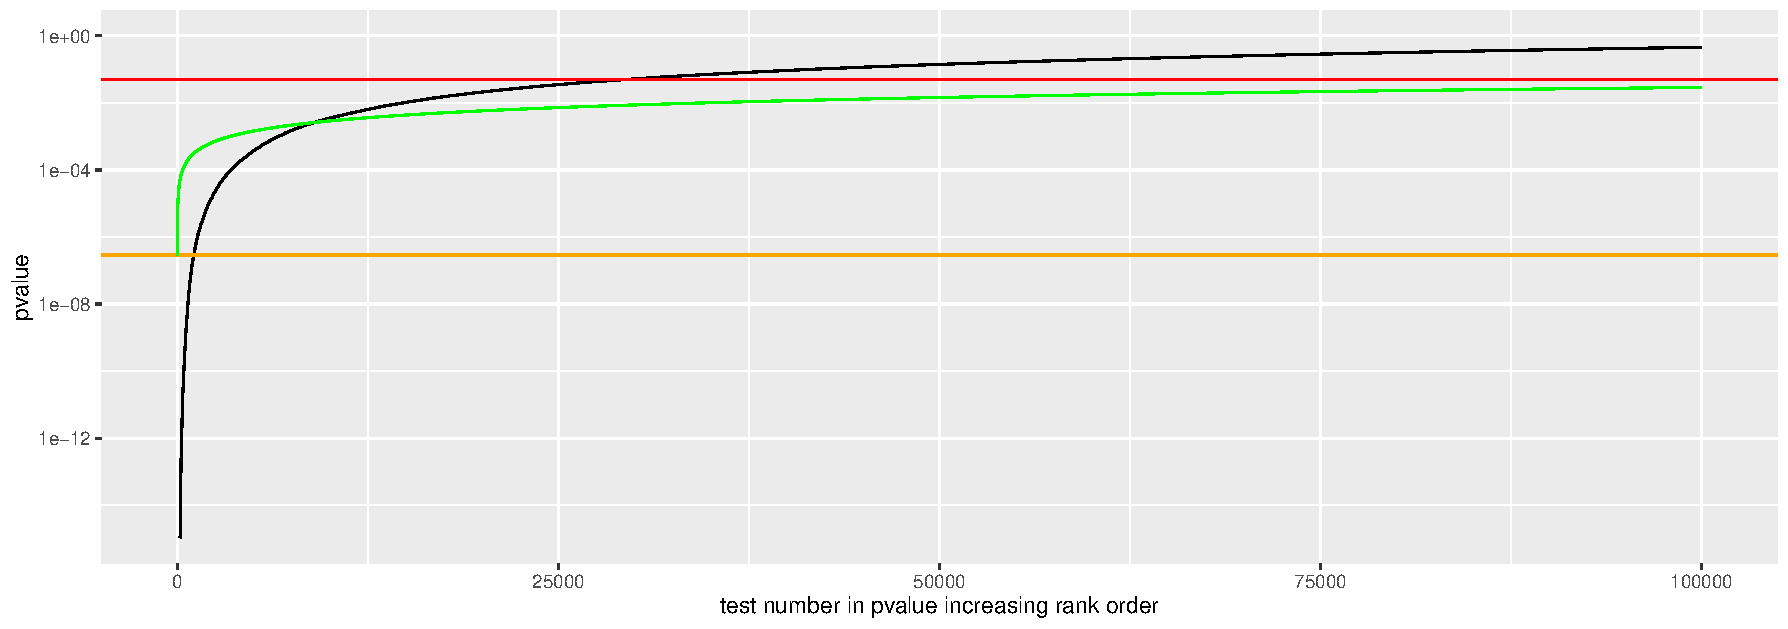
\includegraphics[width=7in]{pvals}
\end{figure}}~\spc{1}

\easysubproblem{Compute the Bonferroni and Sidak $\alpha$ thresholds. Ensure that the Bonferroni is smaller than the Sidak.}\spc{4}

\easysubproblem{The Simes $\alpha$ threshold is 0.00262. Would that yield more rejections than Bonferroni? Yes / No.}\spc{-0.5}

\easysubproblem{Employing the Benjamini-Hochberg procedure, what does your number of rejections mean? Explain and be specific.}\spc{3}

\intermediatesubproblem{Why do you think the Benjamini-Hochberg procedure to control FDR has had such a huge impact on science?}\spc{3}

\easysubproblem{We looked at the illustration below during lecture, the histogram of the pvals. 

\begin{figure}[h]
\centering
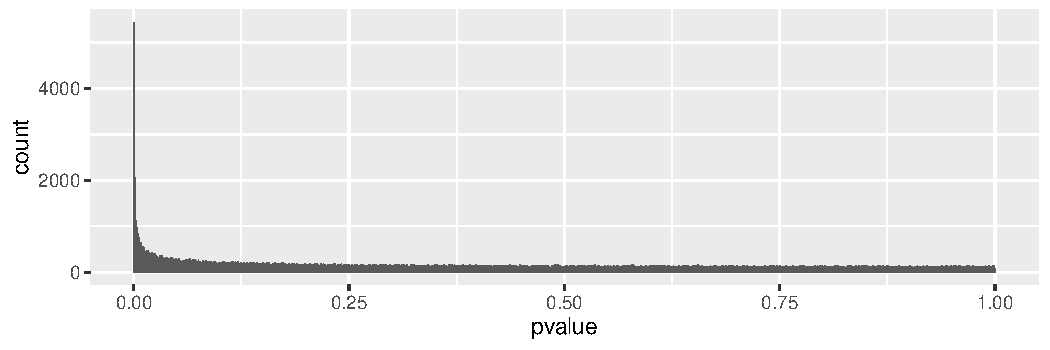
\includegraphics[width=7in]{hist_pvals}
\end{figure}

Do you believe that all $H_0$'s are true? Yes / No.}\spc{-0.5}

\hardsubproblem{Do you think that Bonferroni / Sidak / Simes are more conservative now that you've seen the plot? Explain}\spc{3}


\end{enumerate}%%%


\pagebreak

\problem{This problem will cover the Wald Test for the MLE, the Score Test and the Likelihood Ratio Test when testing the parameter in the iid Bernoulli DGP. Consider the MLE, $\thetahatmle = \Xbar$ and the null hypothesis $H_0: \theta = \theta_0$. We know by the central limit theorem (and also by the asymptotic normality of the MLE theorem) that under $H_0$ the standardized sampling distribution denoted $Z$ is asymptotically normal:

\beqn
Z = \frac{\Xbar - \theta_0}{\sqrt{\overn{\theta_0 (1 - \theta_0)}}} \convd \stdnormnot
\eeqn
}

\noindent Since the Wald test is defined as a z-test based on an asymptotically normal estimator, the $Z$ above is the estimator for the Wald test. And thus the 1-proportion z-test is the Wald test in this setting. 

Below are critical values for the chi-squared distribution that will be of use throughout the rest of the homework:

\begin{table}[ht]
\tiny\tt
\centering
\begin{tabular}{r|rrrrrrrrrrrrrrrrrrrr}
df & 1 & 2 & 3 & 4 & 5 & 6 & 7 & 8 & 9 & 10 & 11 & 12 & 13 & 14 & 15 & 16 & 17 \\ 
  \hline
$F_{\chisq{df}}(\cdot) = 95\%$ & 3.84 & 5.99 & 7.81 & 9.49 & 11.07 & 12.59 & 14.07 & 15.51 & 16.92 & 18.31 & 19.68 & 21.03 & 22.36 & 23.68 & 25.00 & 26.30 & 27.59  \\ 

\end{tabular}
\end{table}
\begin{enumerate}

\easysubproblem{The data is $n = 100$ and $\xbar = 61$. We are testing against $H_0: \theta = \half$. Show that the Wald test statistic (the estimate) is $z = 2.2$. Would you reject the null hypothesis at $\alpha = 5\%$ using the Wald test?}\spc{3}

\easysubproblem{If you square the Wald test statistic, you get an equivalent test

\beqn
Z^2 = \frac{(\Xbar - \theta_0)^2}{{\overn{\theta_0 (1 - \theta_0)}}} \convd \chisq{1}
\eeqn

Some textbooks define this as Wald test. Compute the test statistic (the estimate) for the data in (a) and show you reach the same decision in your hypothesis test.}\spc{3}

\easysubproblem{Prove the Score test for one parameter for any iid DGP $f(x;\theta)$, i.e., declare the estimator and provide its exact or approximate distribution (lecture 19).}\spc{10}


\intermediatesubproblem{Show that the score test is equivalent to the Wald test in the case where the DGP is iid $\bernoulli{\theta}$. This means the estimator is the same. For all the formulas you need, see middle of lecture 10 where we derived $I(\theta)$ for the iid $\bernoulli{\theta}$ DGP. Then it's algebraic simplication from there.}\spc{8}

\easysubproblem{Prove the Likelihood Ratio (LR) test for one parameter for any iid DGP $f(x;\theta)$, i.e., declare the estimator and provide its exact or approximate distribution (lec 20).}\spc{12}

\easysubproblem{Show that the LR test is \emph{not} equivalent to the Wald test / Score test in the case where the DGP is iid $\bernoulli{\theta}$. This means the estimator is \emph{not} the same. This is marked easy because it appears at the end of lecture 19.}\spc{7}

\easysubproblem{Compute the test statistic (the LR test statistic which we denote $\doublehat{\Lambda}$ in lecture) for the data in (a). Since the likelihood ratio test is not the same as the Wald test, your answer should be different than the answer in (b). But since the Wald, Score and Likelihood Ratio tests are all asymptotically equivalent, this means the answer here should be \emph{approximately} the same numeric value as the answer you got in (b). Does the difference in value change your decision (do you still retain/reject $H_0$ as you did previously)?}\spc{3}


\easysubproblem{Plot a log-likelihood function vs $\thetahathat$. Mark $\thetahathatmle$ and $\theta_0$, a value you're testing aginst in $H_a$. Also illustrate the distance $wa$ that corresponds to the numerator of the statistic used in the Wald test for the MLE, the distance $sc$ that corresponds to the numerator of the statistic used in the score test and $lr$ which corresponds to half the likelihood ratio statistic.}\spc{11}


\extracreditsubproblem{Prove the asymptotic equivalence of the Wald, Score and LR tests.}\spc{1}
\end{enumerate}%%%


\problem{We will talk about the generalized Likelihood Ratio test here for testing the difference between a \emph{full model} and a \emph{reduced model} where the DGP is shared between the full model and the reduced model and the reduced model is said to be \emph{nested in} the full model.

Consider the generalized logistic DGP:

\beqn
f(x; \theta_1, \theta_2, \theta_3) = \frac{
\theta_3 e^{-\frac{x - \theta_1}{\theta_2}}
}{
\theta_2 \tothepow{
1 + e^{-\frac{x - \theta_1}{\theta_2}}
}{\theta_3 + 1}
}
\eeqn

\indent The reason why it's called the \qu{generalized} logistic model is because it adds another parameter to the logistic model allowing for more flexibility. }


\begin{enumerate}


\easysubproblem{If we were testing against $H_0: \theta_1 = \theta_{1_0}$ and $\theta_2 = \theta_{2_0}$ and $\theta_3 = \theta_{3_0}$ via the LR test, what would be the asymptotic distribution of $\hat{\Lambda}$? What is the critical threshold value to reject at $\alpha = 5\%$?}\spc{1}

\easysubproblem{If we were testing against $H_0: \theta_1 = \theta_{1_0}$ and $\theta_2 = \theta_{2_0}$ via the LR test, what would be the asymptotic distribution of $\hat{\Lambda}$? What is the critical threshold value to reject at $\alpha = 5\%$?}\spc{1}

\easysubproblem{If we were testing against $H_0: \theta_1 = \theta_{1_0}$ via the LR test, what would be the asymptotic distribution of $\hat{\Lambda}$? What is the critical threshold value to reject at $\alpha = 5\%$?}\spc{1}


\easysubproblem{If we set $\theta_3 = 1$, the generalized logistic gives us back the vanilla logistic model:


\beqn
f(x; \theta_1, \theta_2, 1) = \frac{
e^{-\frac{x - \theta_1}{\theta_2}}
}{
\theta_2 \tothepow{
1 + e^{-\frac{x - \theta_1}{\theta_2}}
}{2}
}
\eeqn

We wish to test the full model (the generalized logistic) vs the reduced model (the logistic which is the full model restricted to $\theta_3 = 1$). What would be the null hypothesis of this test?}\spc{3}

\hardsubproblem{Derive the LR test statistic $\doublehat{\Lambda}$ for the test in (d) given a sample size $n$ of iid data. Simplify as much as you can. I suggest you use the notation $a, b, c, d, e$, etc for the different maximum likelihood estimates. Remember the MLE's are different in the numerator and the denominator even though they are estimating the same parameter!}\spc{8}


\intermediatesubproblem{For the full model let $\thetahatmle_1$ = 12.22, $\thetahatmle_2$ = 4.03 and $\thetahatmle_3$ = 3.49. For the reduced model let $\thetahatmle_1$ = 18.65 and $\thetahatmle_2$ = 3.09. Let $x_1 = 21.86$ $x_2 = 20.71$ and $x_3 = 16.11$. Although $n=3$ is definitely not a large enough sample size for the asymptotic distribution to kick in, nevertheless compute $\doublehat{\Lambda}$. This will be some boring calculation.}\spc{8}


\intermediatesubproblem{For the JFK windspeed data on midterm 2, question 8, the log-likelihood for the generalized logistic model (the full model) is -1129.654 and the log-likelihood for the logistic model (the reduced model) is -1138.298. Calculate the LR test's statistic $\doublehat{\Lambda}$. Do you reject or retain $H_0$? Can you explain what your rejection or retainment means in a few sentences?}\spc{2}

\end{enumerate}%%%

\problem{This problem is further about the LR test. Below I describe a problem setting that is motivated by Abhinav's question on slack. You do not need to understand what's below and you can skip it if you wish but this is an example of how the LR test is used by real practicing statisticians.

\small \sf
Imagine a clinical trial which is a randomized experiment testing a treatments for depression ($T_1$: therapy vs $C$: no treatment). The usual goal is to measure the \emph{treatment effect}i.e. the difference between these two treatments (which we call $\theta_T - \theta_C$) and then ascertain if the treatment does better than the control (i.e. reject $H_0: \theta_T - \theta_C = 0$). We will be talking about this classic setting during the last two lectures of the course. It is very important outside of clinical trials by the way: Amazon is running 1000's of experiments all the time!

To run the hypothesis test, the standard methodology is linear regression which is taught in ECON 382 and MATH 342. As a secondary goal, we also wish to measure the effect of the subjects' characteristics. In this study we measure ten of them e.g. is this person married? does this person have prior drug usage? how bad was their depression symptoms when the study began? etc. So the total number of parameters in the model is ten plus a intercept to allow for an overall average plus a nuisance parameter for the variance (like we've seen in our testing as well) for a total of 13 parameters.

However, Abhinav was interested in seeing whether the treatment effect differs based on the subjects. To do this test, the standard methodology is to interact the treatment with the ten characteristics creating ten more parameters for a total of 23 parameters (the full model). We then ask the question: is it truly a better explanatory model to add this complexity? Can we get away with having only the original model (which is now termed the reduced model).

\normalsize\rm
}\vspace{-0.4cm}


\begin{enumerate}

\easysubproblem{As described above, the full model has 23 parameters and the reduced model as 13 parameters. We're testing if we need the full model to explain our data. Hence the null hypothesis is that the reduced model is true. What is the approximate distribution of the the LR test statistic $\hat{\Lambda}$?}\spc{0}


\easysubproblem{We fit the models using maximum likelihood and then compute the log likelihoods numericaly. The full model has log likelihood -473.3 and the reduced model has log likelihood -489.2. Run the test and provide your conclusion and write a couple sentences to explain it.}\spc{2}
\end{enumerate}%%%

\end{document}
%%%%%%%%%%%%%%%%%%%%%%%%%%%%%%%%%%%%%%%%%%%
%%%%%%%%%%%%%%%%%%%%%%%%%%%%%%%%%%%%%%%%%%%
%%%%%%%%%%%%%%%%%%%%%%%%%%%%%%%%%%%%%%%%%%%
%%%%%%%%%%%%%%%%%%%%%%%%%%%%%%%%%%%%%%%%%%%
%%%%%%%%%%%%%%%%%%%%%%%%%%%%%%%%%%%%%%%%%%%
%%%%%%%%%%%%%%%%%%%%%%%%%%%%%%%%%%%%%%%%%%%
%%%%%%%%%%%%%%%%%%%%%%%%%%%%%%%%%%%%%%%%%%%

\problem{We will review some Wald tests here.}


\begin{enumerate}


\intermediatesubproblem{For two independent samples of unknown DGP's with means $\theta_1$ and $\theta_2$ and unknown by finite variances, prove that the Wald test is an asymptotically valid 2-sample z-test.

To do this, you technically need a multidimensional \href{https://en.wikipedia.org/wiki/Continuous_mapping_theorem}{continuous mapping theorem} (what we've been calling Thm 5.5.4). So assume that for r.v. sequences $A_n$ and $B_n$ if $A_n \convp a$ and $B_n \convp b$ then $h(A_n, B_n) \convp h(a,b)$ if $h$ is continuous. This looks scary but all you have to do is assume $S_1 \convp \sigma_1$ and $S_2 \convp \sigma_2$ and follow HW4's 1(e) exactly.}\spc{5}

\easysubproblem{For the same obesity study as in 1(b), now consider the outcome metric \qu{binge episodes per week} which is a count metric (e.g. 1 day, 2 days, 3 days, ..., all 7 days!). Explain why the normality assumption does not hold for the DGP in both samples.}\spc{3}

\intermediatesubproblem{Test the theory that mean \qu{binge episodes per week} differs in both poputions. The raw data is in Table 3 and the format is $\xbar \pm s$. Don't forget that standard error is not standard deviation!}\spc{10}

\intermediatesubproblem{Assume a DGP of $\iid \text{Gumbel}(\theta, 1)$. In HW 4 you proved that $\thetahatmle = \natlog{n / \sum_{i=1}^n e^{-X_i}}$ and $I(\theta) = 1$ (the $I(\theta) = e^{-2\theta}$ in lecture 12 was my mistake so please ignore that). Provide the asymptotic distribution of $\thetahatmle$ and run the test from lecture 12 again given the data there.}\spc{7}


\end{enumerate}

\problem{We will discuss theory of confidence intervals here.}


\begin{enumerate}
\easysubproblem{Provide the definition of an interval estimator and interval estimate.}\spc{4}

\easysubproblem{What is the $\prob{\theta \in CI_{\theta, 1-\alpha}}$ if CI refers the interval estimat\inred{or?}}\spc{1}

\hardsubproblem{What is the $\prob{\theta \in CI_{\theta, 1-\alpha}}$ if CI refers the interval estimat\inred{e?}}\spc{4}

\intermediatesubproblem{Let's say you run $L = 37$ experiments where you compute an exact $CI_{\theta, 1-\alpha}$ in each one. What is the probability none of the confidence intervals contain $\theta$?}\spc{5}

\intermediatesubproblem{Find an approximate $CI_{\theta, 1-\alpha}$ by inverting the Wald test of 2(d). This means you must prove the approximate coverage is valid.}\spc{10}

\intermediatesubproblem{For the same obesity study as in 1(b), consider the outcome metric \qu{binge episodes per week}, define $\theta_1$ and $\theta_2$ as the unknown populations' mean parameter and find an exact $CI_{\theta_1 - \theta_2, 1-\alpha}$ assuming both population DGP's are normal and $\sigsq$ is the same in both populations.}\spc{4}

\intermediatesubproblem{For the same obesity study as in 1(b), consider the outcome metric \qu{binge episodes per week}, define $\theta_1$ and $\theta_2$ as the unknown populations' mean parameter and find an approximate $CI_{\theta_1 - \theta_2, 1-\alpha}$ assuming both population DGP's are normal and $\sigsq$ is \emph{not} the same in both populations.}\spc{4}

\intermediatesubproblem{For the same obesity study as in 1(b), consider the outcome metric \qu{binge episodes per week}, define $\theta_1$ and $\theta_2$ as the unknown populations' mean parameter and find an approximate $CI_{\theta_1 - \theta_2, 1-\alpha}$ \emph{without} assuming both population DGP's are normal.}\spc{4}

\end{enumerate}


\problem{We will talk a little statistical philosophy here.}


\begin{enumerate}
\easysubproblem{For a single point estimate, what can a skeptic of the field of Statistics argue?}\spc{2}

\easysubproblem{For a single hypothesis test result, what can a skeptic of the field of Statistics argue?}\spc{3}

\hardsubproblem{For the previous question, consider the case where $H_0$ is rejected, if the $p$-value is 1 in 1,000,000,000, does the skeptic have any argument? Thanks to Robin for making me think about this.}\spc{4}

\easysubproblem{For a single confidence interval estimate, what can a skeptic of the field of Statistics argue?}\spc{1}

\easysubproblem{How do you define \qu{wrong} in point estimation?}\spc{1}
\easysubproblem{How do you define \qu{wrong} in confidence interval construction?}\spc{1}
\easysubproblem{How do you define \qu{wrong} in hypothesis testing?}\spc{1}

\end{enumerate}


\problem{In this question, we will use the \emph{univariate delta method} and \emph{multivariate delta method}.}


\begin{enumerate}


\easysubproblem{State the univariate delta method. List assumptions.}\spc{5}

\easysubproblem{Prove the univariate delta method. Justify each step.}\spc{7}

\hardsubproblem{Assume the $\iid$ Bernoulli DGP with mean $\theta$. Sometimes researchers are interested in a different parameterization, the log odds against the event ocurring, i.e. $\natlog{\frac{1-\theta}{\theta}}$, a metric that can be any number in $\reals$. Derive an asymptotically normal estimator for the log odds.}\spc{8}

\easysubproblem{Given the previous answer, write a formula for $CI_{\phi, 1-\alpha}$ where $\phi$ is the log odds against the event ocurring.}\spc{8}

\intermediatesubproblem{Recall the PUFA-Atrial Fibrilation after open heart surgery \href{https://www.onlinejacc.org/content/45/10/1723}{study} from many of our lectures (especially lecture 14). In class we derived a confidence interval for the odds against getting Atrial Fibrilation in the control group. Compute a $CI_{\phi, 95\%}$ where $\phi$ is the log odds against getting Atrial Fibrilation in the control group and round to 3 digits.}\spc{3}


\easysubproblem{State the multivariate delta method. List assumptions.}\spc{5}

\extracreditsubproblem{Prove the multivariate delta method. Justify each step.}\spc{12}


\hardsubproblem{Assume two independent populations both with $\iid$ DGP's with means $\theta_1$, $\theta_2$ respectively and variances $\sigsq_1$ and $\sigsq_2$ respectively. Using the multivariate delta method, derive an asymptotically normal estimator for the ratio of the means $\frac{\theta_1}{\theta_2}$.}\spc{8}

\intermediatesubproblem{Given the previous answer, write a formula for $CI_{\phi, 1-\alpha}$ where $\phi$ is the ratio of the means $\frac{\theta_1}{\theta_2}$.}\spc{4}

\intermediatesubproblem{For the same obesity study as in 1(b), consider the outcome metric \qu{binge episodes per week}, define $\theta_1$ and $\theta_2$ as the unknown populations' mean parameter and find an approximate $CI_{\phi, 1-\alpha}$ where $\phi$ is the ratio of the means $\frac{\theta_1}{\theta_2}$.}\spc{4}

\hardsubproblem{List all the reasons why the CI you constructed in the previous problem is approximate. How much should you trust it?}\spc{6}
\end{enumerate}


\problem{We will review (a) the equivalence of the two-sided $z$ test and the $\chi^2$ test and (b) the equivalence of the two-sided $t$ test and the $F$ test.}


\begin{enumerate}


\easysubproblem{Fill in the blank:

\beqn
\frac{\thetahat - \theta}{\mathbb{S}\text{E}[\thetahat]} \convd \stdnormnot \mathimplies \frac{(\thetahat - \theta)^2}{\mathbb{V}\text{ar}[\thetahat]} \convd 
\eeqn}~\spc{-0.5}

\easysubproblem{Fill in the blank:

\beqn
\sqrt{n}\frac{\thetahat - \theta}{S} \sim T_{n-1} \mathimplies n\frac{(\thetahat - \theta)^2}{S^2} \sim 
\eeqn}~\spc{-0.5}

\easysubproblem{For the PUFA-Atrial Fibrilation after open heart surgery \href{https://www.onlinejacc.org/content/45/10/1723}{study}, test the hypothesis that AF incidence is unequal between the PUFA and non-PUFA groups using an approximate $\chi^2$ test at $\alpha = 5\%$.}~\spc{5}

\end{enumerate}


\problem{This example is a famous one and you can find it on p161 of AoS. \href{https://en.wikipedia.org/wiki/Gregor_Mendel}{Gregor Mendel} was a scientist and abbott in what's now modern-day Czech Republic. In 1866 he published his work on a theory of genetic inheritance. He conjectured that if phenotypes, i.e. what you can see in an organism, were binary (e.g. ear lobe attached to your face or separated from the face) it was controlled by a pair of \qu{genes}. He proposed that the constituents of the pairs were either \qu{recessive} or \qu{dominant}. If one or both were dominant, the dominant phenotype would be expressed. If both were recessive, the recessive phenotype would be expressed. See \href{https://en.wikipedia.org/wiki/Gregor_Mendel\#/media/File:Mendelian_inheritance.svg}{this illustration}.

In his famous pea experiment, he looked at two binary phenotypes of peas: shape (round vs. wrinkled) and color (yellow vs. green) which he assumed independent. He conjectured that the round was the dominant shape and yellow was the dominant color. He also conjectured that the initial expression of the genes were 50-50 dominant recessive. Thus, you would get 3/4 of the peas be round (dominant-dominant, dominant-recessive, recessive-dominant), 1/4 of the peas be wrinkled (recessive-recessive only), 3/4 of the peas be yellow (dominant-dominant, dominant-recessive, recessive-dominant) and 1/4 of the peas be green (recessive-recessive only). 

Putting it all together, 9/16 of all peas should be yellow and round, 3/16 should be yellow and wrinkled, 3/16 should be green and round and only 1/16 should be green and wrinkled. Between 1856 and 1863 he sampled $n = 556$ peas growing in his garden.}


\begin{enumerate}


\intermediatesubproblem{Formulate Mendel's conjecture as a null and alternative hypothesis. Construct your own notation.}\spc{2}

\easysubproblem{Assuming the null hypothesis, what are the expected counts in each of the four groups for the $n = 556$ peas?}\spc{2}

\easysubproblem{Of the $n = 556$ peas, he found 315 were yellow and round, 101 were yellow and wrinkled, 108 were green and round and 32 were green and wrinkled. Calculate the value of the $\chi^2$ goodness-of-fit test statistic to two digits which gauges the data's departure from $H_0$.}\spc{8}

\easysubproblem{Run \qu{Pearson's $\chi^2$ goodness of fit test} at $\alpha = 5\%$ and state whether there is sufficient evidence to reject Mendel's theory of genetic inheritance.}\spc{0.5}

\end{enumerate}


\problem{In class we spoke about the relationship between hair color and eye color for men. Here is an analogous dataset for women:

\begin{table}[ht]
\centering
\begin{tabular}{rrrrr}
  \hline
 & Brown & Blue & Hazel & Green \\ 
  \hline
Black & 36 & 9 & 5 & 2 \\ 
  Brown & 66 & 34 & 29 & 14 \\ 
  Red & 16 & 7 & 7 & 7 \\ 
  Blond & 4 & 64 & 5 & 8 \\ 
   \hline
\end{tabular}
\end{table}

}


\begin{enumerate}


\easysubproblem{Write the null hypothesis for hair and eye color being independent.}\spc{1}

\intermediatesubproblem{Under the null hypothesis, \emph{estimate} the expected frequencies in all 16 groups.}\spc{5}

\intermediatesubproblem{Calculate the $\chi^2$ test statistic which gauges the data's departure from $H_0$.}\spc{3}

\intermediatesubproblem{Run a chi-squared test of hair and eye color being independent at $\alpha = 5\%$.}\spc{0.5}


\hardsubproblem{[MA] There is also a \qu{chi-squared test of homogeneity}. Here we are testing the equality of proportion among many groups at once. If there was only one group, then you would use a two-proportion z-test. It turns out the test statistic is the same and it is asymptotically $\chi^2$ with degrees of freedom being the number of tests minus 1 (just like in the setting of the goodness of fit test). Here's frequency data on men and women's hair color:

\begin{table}[ht]
\centering
\begin{tabular}{rrrrr}
  \hline
 & Brown & Blue & Hazel & Green \\ 
  \hline
Male & 98 & 101 & 47 & 33 \\ 
  Female & 122 & 114 & 46 & 31 \\ 
   \hline
\end{tabular}
\end{table}

Write $H_0$ homogeneity between male and female across hair colors and $H_a$: heterogeneity between male and female across hair colors using this class's canonical notation. Then run the test.}\spc{15} 

\end{enumerate}

\problem{Herein we will practice the model selection theory and techniques we learned in class. Consider the following dataset with $n=10$: -0.67, -0.58,  0.57, -0.34, -0.22,  0.60, -0.42, -0.01,  0.76,  0.80. Consider the following $M=4$ candidate iid DGPs / models similar to the lecture:

\begin{itemize}
\item[MOD 1:] $ \normnot{\theta_1}{\theta_2}$
\item[MOD 2:] $ \text{Cauchy}(\theta_1, \theta_2)$
\item[MOD 3:] $ \text{Logistic}(\theta_1, \theta_2)$
\item[MOD 4:] $ \text{Laplace}(\theta_1, \theta_2)$
\end{itemize}

\noindent After using maximum likelihood, we find the following estimates and AIC metrics for each DGP / model:

\begin{itemize}
\item[MOD 1:] $ \normnot{0.050}{0.303}$. AIC = 20.427
\item[MOD 2:] $ \text{Cauchy}(-0.182, 0.391)$. AIC = 26.899
\item[MOD 3:] $ \text{Logistic}(0.028, 0.345)$. AIC = 21.689
\item[MOD 4:] $ \text{Laplace}(-0.176,0.496)$. AIC = 23.843
\end{itemize}

}


\begin{enumerate}


\intermediatesubproblem{Compute $\ell\parens{\thetahathatmle_1, \thetahathatmle_2; x_1, \ldots, x_{10}}$ for MOD 1. This is nothing but some computation. Remember $\theta_2$ in the $ \normnot{\theta_1}{\theta_2}$ notation is the variance not the standard deviation!}\spc{5}


\intermediatesubproblem{[MA] Compute $\ell\parens{\thetahathatmle_1, \thetahathatmle_2; x_1, \ldots, x_{10}}$ for MOD 3.}\spc{5}

\easysubproblem{Compute the AIC for MOD1 given your answer in (a). Is it the same that I computed using software?}\spc{3}


\easysubproblem{According to the AIC metric, which model fits this dataset the best?}\spc{1}

\easysubproblem{Calculate the $M=4$ Akaike weights. If the true model was among these four candidate models, what is the probablity the true model is normally distributed?}\spc{3}

\easysubproblem{Compute all AICc metrics. According to the AICc metric, which model fits this dataset the best?}\spc{3}

\easysubproblem{Why should AICc be employed in this case instead of AIC?}\spc{3}

\extracreditsubproblem{Prove the bias term from the lecture is $K_m$. State all assumptions}\spc{3}
\end{enumerate}


\end{document}

%%%%%%%%%%%%%%%%%%%%%%%%%%%%%%%%%%%%%%%%%%%%%%%%%%%%%%%%%%%%%%%%%%%%%%%%